%!TEX root = ../../../adrien_gomar_phd.tex
\chapter{Presentation of the toy problems}
\label{cha:toy_problems}

\chabstract{In this chapter, three toy problems are
set up to thoroughly study the properties
of the chosen harmonic balance approach. The first
toy problem is the resolution of the periodic linear advection
equation. An
analytic solution is known, allowing to accurately assess
the harmonic balance method from a theoretical point of view.
The second toy problem is a channel flow with an
oscillating back-pressure. It is solved using the 2D Navier--Stokes
equations. This allows to highlight the properties of the harmonic
balance method in a non-linear equation framework. 
Finally, the third toy problem is a model problem of a turbomachinery configuration.
A Gaussian function representative of a wake is injected and convected through
the domain using the 3D Euler equations. This test case
will be used to assess the specific problems arising when using
the harmonic balance approach in turbomachinery computations.
Furthermore, 
the solver used for these last two cases is the \emph{elsA}
code which will be used for the CROR applications.}

\minitoc
\newpage


\section{Periodic linear advection}
\label{sec:toy_convection}
%!TEX root = ../../../adrien_gomar_phd.tex

To properly assess the convergence of harmonic balance computations,
a model problem is set up. The constant convection 
equation is numerically solved within a harmonic balance 
framework. The convection equation is
\begin{equation}
  \label{eq:convection}
  \frac{\partial u}{\partial t} + c \frac{\partial u}{\partial x} = 0,
\end{equation}
where $c$ denotes the constant convection speed and $u$ the velocity. 
It is chosen for two reasons: first, the constant
convection equation is a simple unsteady 
linear partial differential equation
and second, a straightforward analytical solution
exists
which ease the analysis of the numerical solutions. In fact,
it only depends on the boundary conditions:
\begin{equation}
  \label{eq:solconvanalytic}
    u(x, t) = u(x=0, x/c + t) = u_0 (x/c + t),
\end{equation}
where $u_0(t) = u(x=0, t)$ is the temporal evolution of 
the boundary condition ($x=0$). 
The size of the domain is $L_x$ and the number of grid points is
proved to be converged for $2,000$ nodes.

The convection equation is solved within the harmonic
balance framework in time using a finite difference approach
in space.
A $4$\textsuperscript{th} order centered finite
difference scheme is used to evaluate the spatial derivative:
\begin{equation}
    \frac{\partial u}{\partial x} (x = x_i, t=t_q) \approx 
    \frac{-u^{i+2}_{q} + 8 u^{i+1}_{q} - 8 u^{i-1}_{q} + u^{i-2}_{q}}{12\Delta x},
    \label{eq:convection_center4}
\end{equation}
where $u_q^i$ is the concatenation of the velocity for  
all the HB instants,
evaluated at position $i$ within pseudo-iteration $q$.
A four step Runge-Kutta method is then use to time 
march the equation to the steady state with the coefficients $\alpha_0 = 0$,
$\alpha_1 = 1/4$, $\alpha_2 = 1/3$, $\alpha_3 = 1/2$ and $\alpha_4 = 1$.
The k\textsuperscript{th} step is evaluated by:
\begin{equation}
    u_k = u_q - \alpha_k \Delta t \left [ 
          c \frac{\partial u_{k-1}}{\partial x} (t=t_q + \alpha_{k-1} \Delta t)
          + D_t(u_k)
          \right],
    \label{eq:convection_rk4}
\end{equation}
where the HB source term $D_t(u_k)$ is computed using 
Eq.~\eqref{eq:sm_hb_mono_source_term_analytic} if the mono-frequential
formulation is used or Eq.~\eqref{eq:sm_multi_spectral_operator}
for the multi-frequential formulation.
As we use 
an explicit time marching scheme, the CFL number is set to $1$ to ensure stability.

A function is periodically injected at the left boundary
condition~$u_0$.
In this paper, the following functions will be
investigated: a sum of sine functions, a rectangular
function and a Gaussian function. All of these lasts are periodized
using a periodic operator defined as:
\begin{equation}
    \text{period} \colon
    \begin{cases}
        [0: \infty] & \longmapsto[-T/2: T/2]\\
        t & \longmapsto \displaystyle - \frac{T}{2} + t \pmod T,
    \end{cases}
    \label{eq:periodic_operator}
\end{equation}
where $T$ is the period of the unsteady phenomenon. This period 
is chosen so that, when the frequency of the 
phenomenon is set to $1$, only one pattern of the function 
appears at a time in the domain.
This is done by setting $T$ to:
\begin{equation}
   T = \frac{L_x}{c},
   \label{eq:time_spatial_correspondence}
\end{equation}
where $L_x$ is the size of the domain and $c$ the convection speed.

For the right boundary condition, imposing a periodicity condition is
numerically stiff. For this reason, the scheme is degenerated 
to an upwind scheme to avoid wave reflections. It is degenerated to
a 2\textsuperscript{nd} order scheme on the second to last cell
and to a first order scheme on the last cell:
\begin{align}
    \frac{\partial u}{\partial x} (x = x_{m-1}, t=t_q) &\approx 
    \frac{3 u^{m-1}_{q} - 4 u^{m-2}_{q} + u^{m-3}_{q}}{2\Delta x}, \\
    \frac{\partial u}{\partial x} (x = x_m, t=t_q) &\approx 
    \frac{u^{m}_{q} - u^{m-1}_{q}}{\Delta x},
\label{eq:upwind_scheme}
\end{align}
where $m$ is the total number of grid points.

As an analytical solution is known, it is easy to define the error
made by numerically solving the equation with finite difference.
In particular, the $\mathcal{L}_2$-norm can be defined as:
\begin{equation}
    \frac{\norm{u-u_{analytic}}_2}{\norm{u_{analytic}}_2} = 
    \sqrt{\frac{\sum_{i=0}^{2N} \left[u(t_i) - u_{analytic}(t_i)  \right]^2}{
    \sum_{i=0}^{2N} \left[u_{analytic}(t_i)\right]^2}},
    \label{eq:l2_norm}
\end{equation}
where $t_i$ are the time instants
in which the harmonic balance solution is sought as 
done in Eq.~\eqref{eq:sm_sampling_hb_var}.


\section{Channel flow with oscillating back pressure}
\label{sec:toy_channel}
%!TEX root = ../../../adrien_gomar_phd.tex
\subsection{Presentation of the case}
\label{sub:presentation_of_the_case}

A 2D channel is considered  with a constant left injection
supplemented with a time-varying unsteady back pressure.
As the pressure is oscillating at the outlet, unsteady pressure
fluctuations are created that travel within the flow at the velocity 
$u + c$ and $u - c$, where $u$ denotes 
the local flow velocity and $c$ the sound velocity.
Since the pressure waves are generated at the outlet, only
the $u-c$ waves are seen, resulting in pressure waves propagating
upstream of the channel. Figure~\ref{fig:canal_principle} shows a sketch
of the channel case, illustrating of
the pressure waves.
\begin{figure}[htb]
  \centering
  \includegraphics*[width=0.6\textwidth]{channel_sketch.pdf}
  \caption{Sketch of the channel case.}
  \label{fig:canal_principle}
\end{figure}

\subsection{Numerical setup}

% mesh presentation
It is a 2D channel of length $L_x = 100$~m in the axial
direction and $L_z = 1$~m in the transverse one.
The mesh consists of 1000~points along the axial direction and 10 in the
transverse one, which corresponds to equal spacings in both
directions.

% solver
The \emph{elsA} solver~\cite{Cambier2013} developed by ONERA
is used to solve for the channel flow. Several time-integration schemes
are available: DTS, GEAR, UNS, 
as well as the time-domain harmonic 
balance method implemented by \citet{JSicot2008}. 
This code solves the RANS equations using a cell-centered
approach on multi-blocks structured meshes.

% boundary conditions
The boundary conditions are: (i)~a constant injection condition for the inlet
where the total pressure $p_{i_0}$ and enthalpy $h_{i_0}$ are set,
(ii)~symmetric conditions for the upper and lower bounds as the flow
is assumed to be symmetric in the transverse direction, and (iii)~a
fluctuating static pressure imposed at the outlet:
\begin{equation}
  p_{outlet}(t) = p_m \left[1 + a_1 \sin(2 \pi f_1 t) +
    a_2 \sin(2 \pi f_2 t) \right],
  \label{eq:outlet_canal}
\end{equation}
where $p_m$ is the temporal average static pressure, $a_n$ the
amplitude of the $n$\textsuperscript{th} mode and $f_n$ its
frequency.
The mean velocity of the flow is imposed through a
static pressure condition $p_m$ at the outlet:
\begin{equation}
    p_m = \frac{p_{i_0}}{\left(1 + 
    \frac{\gamma - 1}{2} M_{\inf}^2 \right) ^ {\frac{\gamma}{ \gamma - 1}}} ,
\end{equation}
the mean velocity is thus set by imposing the
target mean Mach number value $M_{\inf}$.
At the azimuthal boundaries, phase-lag conditions~\cite{Erdos1977} 
are used to take into account for the space-time periodicity.

% numerical schemes
This configuration is turbulent as the Reynolds number based on the
inlet flow velocity and the axial length of the channel is about $R_e
\approx 2.0 \times 10^9$.  Turbulence is modeled using the
one-equation model of \citet{Spalart1992}, and the
third-order upwind \citet{Roe1981} scheme is used to compute the
convective fluxes.

\subsection{Validation of the toy problem}
An analytical solution is provided by \citet{Merkle1987} for
incompressible flows. This has been used by \citet{McMullen2001}
to validate the implementation of their NLFD approach.
However, this toy problem is used
to assess the properties of the harmonic balance within
the Navier--Stokes equations framework. Therefore,
this analytical solution will not be used and the validation of
this tool will rely on classical time-marching, namely DTS, solutions.


\section{Model turbomachinery configuration}
\label{sec:model_tbm}
%!TEX root = ../../../adrien_gomar_phd.tex
\subsection{Numerical Setup}
We consider a simplified configuration modeling a turbomachinery 
stage. The configuration consists of a spatially 
periodic azimuthal perturbation advected downstream 
of the inlet boundary of the computational domain. 
The domain is made of two grid blocks in relative 
motion, so that the perturbation, which is steady 
in the upstream block, is seen as unsteady by the 
downstream one, and is thus representative of 
turbomachinery wakes advected across an inter-wheel interface.
The blocks are generated in cylindrical
coordinates such that the presented configuration
can be assimilated to a slice of 
a turbomachinery stage.
Without loss of generality, 
we set the rotation velocity of the upstream block to zero (stator). 
The stator is composed of $B_{stator} = 10$
"virtual" blades and the rotor by $B_{rotor} = 12$ "virtual" blades.
These are termed virtual blades as no blade is actually meshed.
This is a typical pitch ratio encountered 
in contra-rotating open rotor applications in which 
the first row contains more blades 
than the second (see Sec.~\ref{sec:CROR}). Indeed, in
these applications, the number
of blades is typically smaller than classical
turbomachinery configurations. %This means that a wake
% with a given width will be seen thinner because of the bigger
% relative pitch. 

A wake is axially injected at the inlet of the
stator block following the Lakshminarayana and
Davino
similarity law defined in Eq.~\eqref{eq:similarity}.
It is schematically represented in 
Fig.~\ref{fig:rotating_blocks}.
This is thus a representative model problem of the wake shed
by an upstream row that crosses the rows interface, 
here the stator-rotor interface.

The flow is modeled through the 
Euler equations in order to avoid wake thickening
associated with viscous effects. 
The velocity is not imposed at the inlet directly
but rather through the total pressure and total enthalpy distributions:
\begin{equation}
  \label{eq:rotatingblocks_ptot}
    p_{i0} (\theta) = p_{i_{ref}} \left[1 - 
        \Delta p_i \cdot e^{
          -0.693 \left( 2 \frac{\theta}{L} \right) ^ 2}\right],
\end{equation}
\begin{equation}
  \label{eq:rotatingblocks_htot}
    h_{i0} (\theta) = h_{i_{ref}} \left[1 - 
        \Delta h_i \cdot e^{
          -0.693 \left( 2 \frac{\theta}{L} \right) ^ 2}\right],
\end{equation}
where $p_{i0}$ is the inlet total pressure, $\Delta p_i$ the total pressure
deficit in the wake,
$h_{i0}$ the inlet total enthalpy, $\Delta h_i$ the total enthalpy
deficit in the wake and $L$ the wake width.
% As the total enthalpy and total pressure deficits are not
% easy to define, they are estimated from a turbomachinery
% simulation. The idea here is to impose a distortion that
% is physical. This does not remove any generality
% to the current approach.
To impose a realistic distortion, the total pressure and
enthalpy deficits are estimated from a separate turbomachinery simulation.
This leads to $\Delta p_i = 0.025$ and 
$\Delta h_i = - 0.007$.
The negative sign is due to overturning in the wake, which
is due to velocity composition, and therefore specific to rotors.
The static pressure $p_{s_1}$ is imposed at the outlet:
\begin{equation}
    p_{s_1} = \frac{p_{ref}}{\left(1 + 
    \frac{\gamma - 1}{2} M_{ref}^2 \right) ^ {\frac{\gamma}{ \gamma - 1}}} ,
\end{equation}
the mean velocity is thus set by imposing the
target mean Mach number value $M_{ref}$.
At the azimuthal boundaries, phase-lag conditions~\cite{Erdos1977} 
are used to take into account for the space-time periodicity. %, 
% allowing to compute only a single blade passage, 
% as explained in Sec.~\ref{sec:turbomachinery_adaptation}.

Roe's scheme~\cite{Roe1981} with second-order MUSCL extrapolation 
is used for the spatial discretization of
the convective fluxes, and an implicit backward Euler scheme is used
to march the HB equations in pseudo-time.

A parametric study is carried out over the two parameters 
that influence the truncation error as defined in 
Eq.~\eqref{eq:def_truncation_error}: the number of harmonics and the wake width.
The number of harmonics used for the computations ranges from 1 to $25$.
%in order to ease 
%the post processing but 
%Note that a harmonic balance simulation represents $2N+1$ steady
%computations coupled together by a source term. This means that the
%equivalent mesh for $N=25$ computation is $(2 * 25 + 1) * 170,000 = 8,670,000$
%grid point mesh, which is large for a reduce order model problem.
The wake width $L$, that drives
Eq.~\eqref{eq:rotatingblocks_ptot} and~\eqref{eq:rotatingblocks_htot} varies
between $1\%$ and $30\%$ according to a logarithmic scale to ease 
the visualization of the results. $375$ computations are performed in total. 

Each grid block has a radial extent of five grid points \emph{i.e.} four cells. 
The azimuthal grid density in the stator and rotor blocks is kept similar
to guarantee a consistent capture of the wake on each side of the interface.
To do so, if $\Delta \theta_{cell}$ denotes the azimuthal length of a cell
at the interface, then:
\begin{equation}
   \Delta \theta_{cell} = \frac{2\pi}{B_{stator}}~\frac{1}{N_{stator}}
   = \frac{2\pi}{B_{rotor}}~\frac{1}{N_{rotor}},
   \label{eq:az_spatial_discretization_1}
\end{equation}
where $N_{stator}$ and $N_{rotor}$ are the number of cells
in the stator and the rotor, respectively. 

% This equation gives finally the relation
% between $N_{stator}$ and $N_{rotor}$ that ensures a uniform azimuthal
% grid density at the interface:
% \begin{equation}
%    12~N_{stator} = 10~N_{rotor}.
%    \label{eq:az_spatial_discretization_2}
% \end{equation}
Mesh convergence for the thinnest wake (1\% of the pitch)
is obtained with 500~cells in the azimuthal direction of
the stator which gives
600~cells for the rotor block.
30~grid points are put in the axial direction. Moreover, a constant
aspect ratio of 5 with respect to the azimuthal length of the cells is
kept, which sets the axial length of the case.
This leads to a total number of grid points of approximately 
170,000. 
Note that the memory requirement of an HB 
simulation is $2N+1$ times that of the equivalent steady case. 
An equivalent steady computation to $N=25$ would 
thus require 
$(2 \times 25 + 1) \times 170,000 = 8,670,000$ grid point mesh.
The grid used for the computations is shown in Fig.~\ref{fig:rotating_blocks}.
\begin{figure}[htb]
  \centering
  \begin{tabular}{cc}
    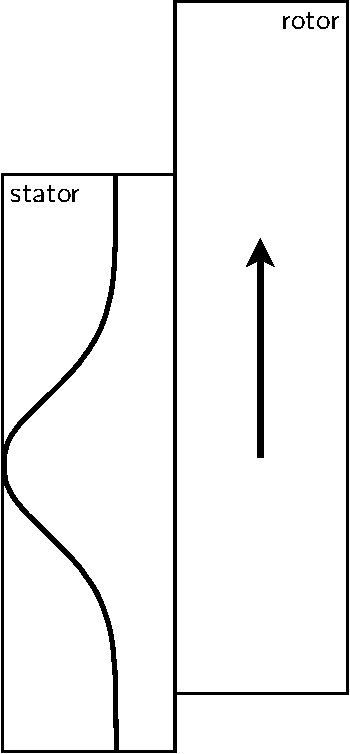
\includegraphics[height=.3\textheight]{ROTATING_BLOCKS.pdf}
    &
    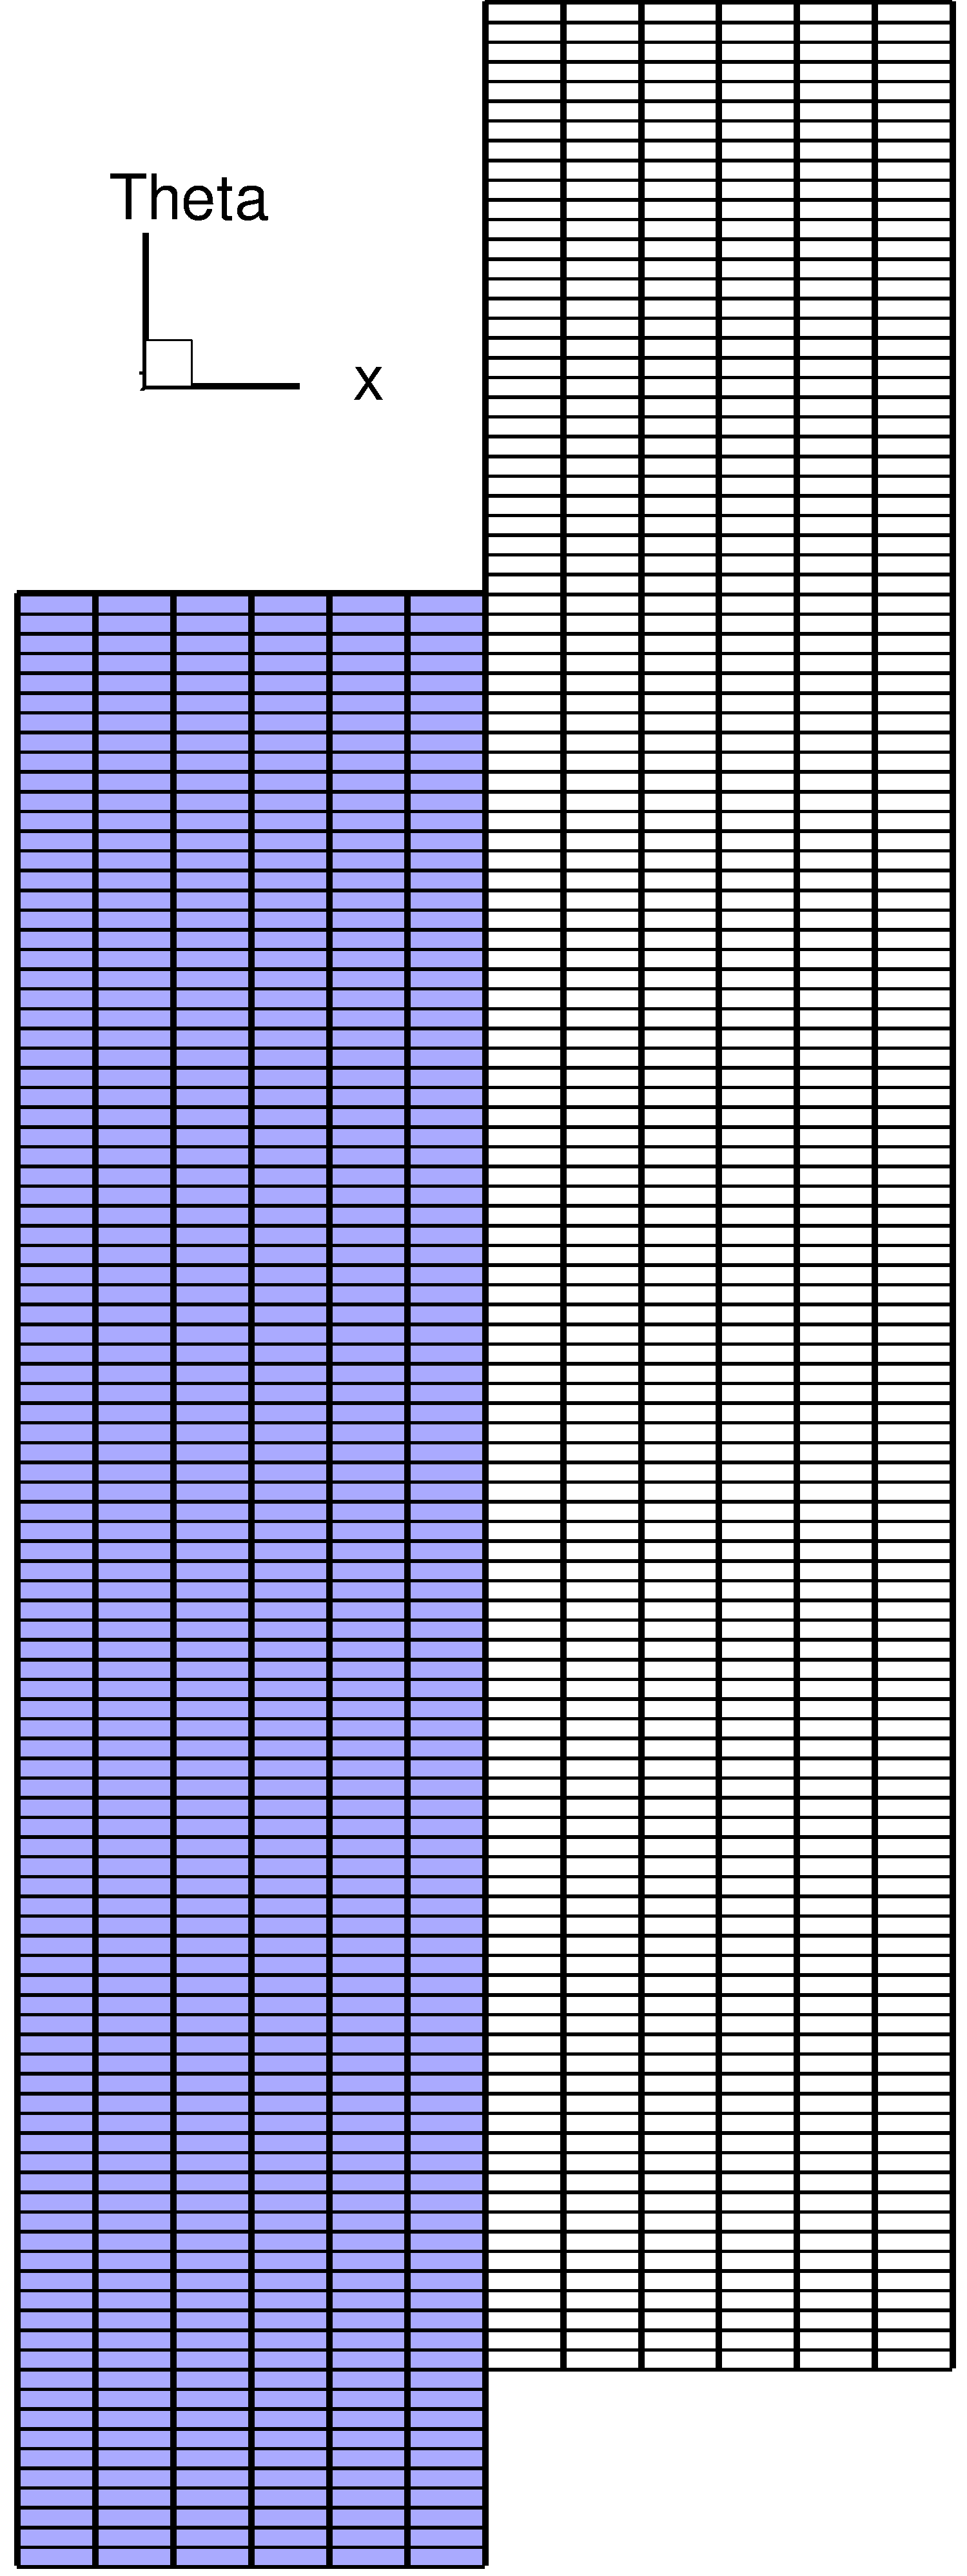
\includegraphics[height=.3\textheight]{RB_mesh_3D.png}\\
    Principle diagram 
    &
    Mesh, one out every five points
  \end{tabular}
\caption{Model turbomachinery configuration.}
\label{fig:rotating_blocks}
\end{figure}
Convergence of the iterative procedure used to solve the HB equations is achieved 
after 3,000 iterations for 
all the simulations. 

\chconclu{}
